\subsection{Circuit Protection}\label{ssec:circuitProtection}
	A important feature of any electronic product/appliance is the immunity against undesired voltage transients. In DAQ systems this is a relevant issue, the inputs of this systems must be protected from possible damage that may be caused by unintentional/accidental high voltage inputs, surges, etc \cite{mathivanan2007pc}.
	\par
	According to \cite{littlelFuseWhatIsTransientVoltage}, Voltage Transients are defined as short duration surges of electrical energy and are the result of the sudden release of energy previously stored or induced by other means. There are many things that can cause voltage transients (commonly refered just by transients) and those can be divided in two groups:

	\begin{itemize}
		\item Repeatable Transients: Usually caused by the operation of inductive loads such as motors, generators and swichting circuits.\label{itm:repeatable-transients}
		\item Random Transients: Uncorrelated transients generated by exclusive events such as lightning, ESD and unpredictable events.\label{itm:random-transients}
	\end{itemize}

	In order to enhance energy efficiency, devices are now operating at lower voltages \cite{xavier2017benefits}. With the miniaturization of electronic components, those have become even more sensitive to electrical stress \cite{littlelFuseWhatIsTransientVoltage}.
	\par
	In automotive environment, many of the supporting electrical components of the vehicle can generate transients, specially from inductive load switching. When the inductive load is switched off, the collapsing magnetic field is converted into electrical energy that turns into a transient \cite{littlelFuseWhatIsTransientVoltage}.

	\subsubsection{Low Pass Filters}\label{sssec:lowPassFilterTransientProtection}
		According to \cite{littlelFuseWhatIsTransientVoltage}, a ESD pulse (fastest common transient pulse) has a overall duration period of less than 100ns (50$\%$ of the peak value) and a rising time that lasts less than 1.2$\mu$s. Figure \ref{fig:esd-test-waveform} shows an example of a ESD Test Waveform.

		\begin{figure}[htbp]
			\centering
			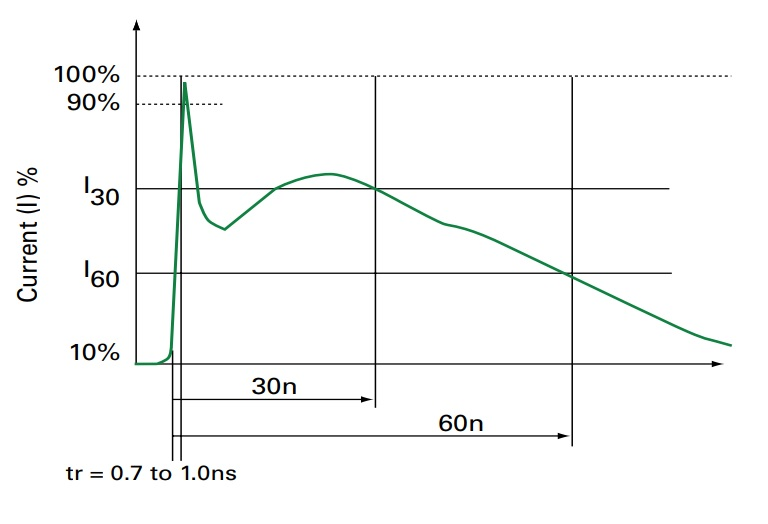
\includegraphics[width=.5\textwidth]{figuras/fig-esd-test-waveform}
			\caption{ESD Test Waveform \cite{esd-test-waveform}}
			\label{fig:esd-test-waveform}
		\end{figure}

		Considering that a signal has a frequency that is lower than the frequency of the transient it is vulnerable to, using a low pass filter to provide suitable attenuation for that transient and still letting the signal frequency on the passaband, it is possible to protect that part of the circuit against this particular transient \cite{standler1988use}. 


	\subsubsection{Transient Voltage Supression Diodes (TVS)}\label{sssec:tvsTransientProtection}

		\subsubsubsection{TVS diodes principle of operation}\label{ssssec:tvsOperation}
			Transient Voltage Supression Diodes or TVS Diodes are the most popular choice for protection components in circuit due to their fast response, low clamping voltage and longevity. Under normal operation TVS diodes are high-impedance devices, interacting as an open circuit to the protected component, during a transient event the TVS diode junction provides a low-impedance path for the transient current \cite{renesasTVS}.
			\par
			There are both uni-directional and bi-directional, the first has an operation curve similar as the one from a Zener diode, during positive transients the device limits the input voltage to it's clamping voltage and during negative transients the spike is clamped to the diode drop. On the other hand, bi-directional TVS diodes are always reverse biased during both negative and positive transients. Figures \ref{fig:uni-tvs-clamp} and \ref{fig:bi-tvs-clamp} show respectively the action of a uni-directional TVS and a bi-directional TVS during transient events.

			\begin{figure}[htbp]
				\centering
				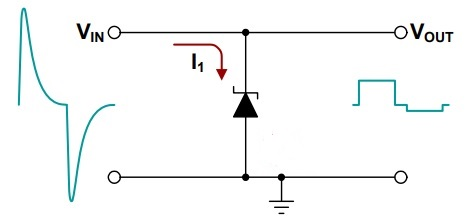
\includegraphics[width=.5\textwidth]{figuras/fig-uni-tvs-clamp}
				\caption{Campling action of a uni-directional TVS \cite{uni-tvs-clamp}}
				\label{fig:uni-tvs-clamp}
			\end{figure}

			\begin{figure}[htbp]
				\centering
				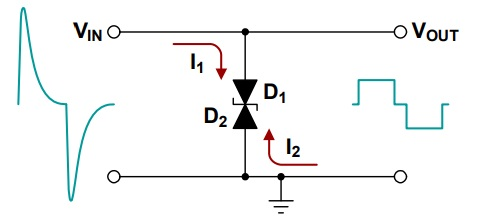
\includegraphics[width=.5\textwidth]{figuras/fig-bi-tvs-clamp}
				\caption{Campling action of a bi-directional TVS \cite{bi-tvs-clamp}}
				\label{fig:bi-tvs-clamp}
			\end{figure}

			\par
			The \textit{Voltage X Current} curve of both uni-directional and bi-directional TVS diodes can be seen repectively on Figures \ref{fig:uni-tvs-curve} and \ref{fig:bi-tvs-curve}.

			\begin{figure}[htbp]
				\centering
				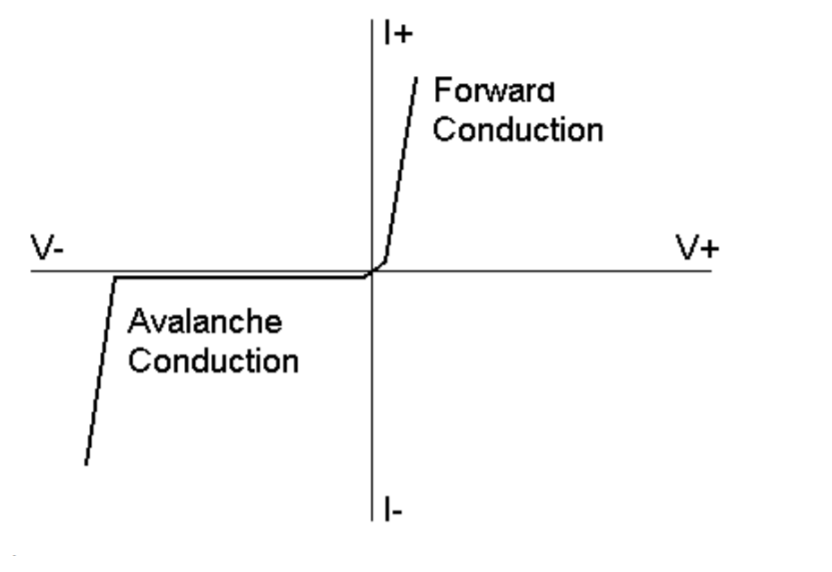
\includegraphics[width=.5\textwidth]{figuras/fig-uni-tvs-curve}
				\caption{\textit{V X I} characteristic of a uni-directional TVS \cite{uni-tvs-curve}}
				\label{fig:uni-tvs-curve}
			\end{figure}

			\begin{figure}[htbp]
				\centering
				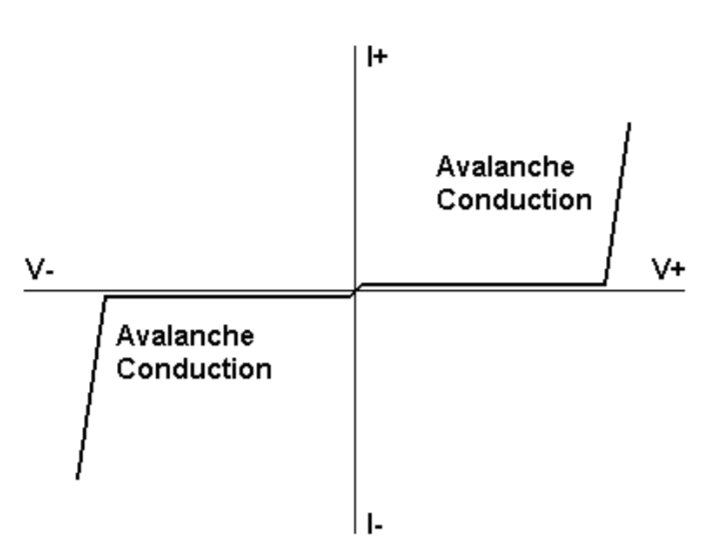
\includegraphics[width=.5\textwidth]{figuras/fig-bi-tvs-curve}
				\caption{\textit{V X I} characteristic of a uni-directional TVS \cite{bi-tvs-curve}}
				\label{fig:bi-tvs-curve}
			\end{figure}

		\subsubsubsection{Selecting TVS Diodes}\label{ssssec:tvsSelection}
		According to \cite{microSemiSelectTVS}, the following parameters of TVS devices are important to consider in order to choose one for protecting a particular circuit net:

		\begin{itemize}
			\item $V_{C}$ (Campling Voltage): the voltage limit that the TVS will allow on the point of intended protection. This voltage should be slightly lower than the point of intended protection absolute maximum voltage rating.\label{itm:campling-voltage}
			\item V$_{WM}$ (Rated Standoff Voltage): this is the maximum voltage in which the TVS still works as a high-impedance device. Therefore, the first step when selecting a TVS device is to know the peak voltage at the point of intended protection during normal operation and then select a TVS device with a appropriate $V_{WM}$.\label{itm:tvs-standoff-voltage}
			\item P$_{PP}$ (Peak Pulse Power): in order to ensure the durability of the TVS device, the maximum power it needs to dissipate should be known. This P$_{PP}$ is calculated by multipling the TVS device $V_{C}$ (Clamping Voltage) and the $I_{PP}$ (Peak Impulse Current, peak current for the transient event).\label{itm:peak-pulse-power}
		\end{itemize}